%-----------------------------------------------------------------------------
%
%               Template for sigplanconf LaTeX Class
%
% Name:         sigplanconf-template.tex
%
% Purpose:      A template for sigplanconf.cls, which is a LaTeX 2e class
%               file for SIGPLAN conference proceedings.
%
% Guide:        Refer to "Author's Guide to the ACM SIGPLAN Class,"
%               sigplanconf-guide.pdf
%
% Author:       Paul C. Anagnostopoulos
%               Windfall Software
%               978 371-2316
%               paul@windfall.com
%
% Created:      15 February 2005
%
%-----------------------------------------------------------------------------


\documentclass[preprint]{sigplanconf}

% The following \documentclass options may be useful:

% preprint      Remove this option only once the paper is in final form.
% 10pt          To set in 10-point type instead of 9-point.
% 11pt          To set in 11-point type instead of 9-point.
% numbers       To obtain numeric citation style instead of author/year.

\usepackage{amsmath}
\usepackage{listings}
\usepackage{color}
\usepackage[normalem]{ulem}

\newcommand{\tool}{\textsc{BigDelta}\xspace}
\newcommand{\fixme} [1] {\textcolor{red}{{\it FIXME}: #1}}
\newcommand{\codefont}[1]{\footnotesize{\texttt{#1}}\normalsize}
\newcommand{\todo} [1]{\textcolor{blue}{{\sf TODO}: #1}}

\definecolor{dkgreen}{rgb}{0,0.6,0}
\definecolor{gray}{rgb}{0.5,0.5,0.5}
\definecolor{mauve}{rgb}{0.58,0,0.82}
\usepackage{times}
\usepackage{array}
\usepackage{url}
\usepackage{float}
\usepackage{subfigure}

\usepackage{pgfplots}
\usepackage{filecontents}
\usetikzlibrary{patterns}
\newcommand{\cL}{{\cal L}}
\lstdefinelanguage{Scala}{
  keywords={typeof, new, true, false, catch,def,val, function, return, null, catch, switch, var, if, in, while, do, else, case, break},
  keywordstyle=\color{blue}\bfseries,
  ndkeywords={class, export,extends, boolean, throw, implements, import, this, abstract},
  ndkeywordstyle=\color{dkgreen}\bfseries,
  otherkeywords={+, =>,<=, ==, >,< , ||},
  identifierstyle=\color{black},
  sensitive=false,
  comment=[l]{//},
  morecomment=[s]{/*}{*/},
  commentstyle=\color{purple}\ttfamily,
  stringstyle=\color{red}\ttfamily,
  morestring=[b]',
  morestring=[b]"
}


\lstset{frame=tb,
  language=Scala,
  aboveskip=3mm,
  belowskip=3mm,
  showstringspaces=false,
  columns=flexible,
  basicstyle={\small\ttfamily},
  numberstyle=\tiny\color{gray},
  keywordstyle=\color{blue},
  commentstyle=\color{dkgreen},
  stringstyle=\color{mauve},
  breaklines=true,
  breakatwhitespace=true,
  tabsize=3,
  numbers=left,
  xleftmargin=2em,
  framexleftmargin=1.5em
}
%!TEX root = paper.tex

\newcommand{\eat}[1]{}

\usepackage{latexsym}
\usepackage{amsfonts}
\usepackage{amsmath}
\usepackage{amssymb}
\usepackage{color}
\usepackage{colortbl}
\usepackage{epsfig}
\usepackage{xspace}
\usepackage{graphicx}
%\usepackage{subfigure}
\usepackage{enumerate}
%\usepackage{enumitem}
%\usepackage{cite}
\usepackage{comment}
\usepackage{stmaryrd}
\usepackage[all]{xy}
%\usepackage{floatrow}
%%%%%%%%%%%%%%%%%%%%%%%%%%%%%%%%%%%%%
%% DO NOT DELETE!!
%%%%%%%%%%%%%%%%%%%%%%%%%%%%%%%%%%%%%
%\usepackage{tikz}
%\usetikzlibrary{trees}

\usepackage[noend]{algorithmic}
\usepackage{algorithm}

\usepackage{epsfig}
\usepackage{multirow}
\usepackage{hhline}
\usepackage{url}
\usepackage[table]{xcolor}
%\usepackage[lined,boxed,vlined,ruled]{algorithm2e}
%\newcommand{\algcct}{\kw{isConsist}^t}
%\newcommand{\algequ}{{\small\kw{EQU}}}

\newcommand{\eq}{\kw{eq}}

\newcommand{\ab}{\allowbreak}

\renewcommand{\algorithmicrequire}{\textbf{Input:}}
\renewcommand{\algorithmicensure}{\textbf{Output:}}

\sloppy
\newcommand\leadsfrom{\mathrel{\reflectbox{\ensuremath{\leadsto}}}}
\newcommand{\rtable}[1]{\ensuremath{\mathsf{#1}}}
\newcommand{\ratt}[1]{\ensuremath{\mathit{#1}}}
\newcommand{\at}[1]{\protect\ensuremath{\mathsf{#1}}\xspace}
\newcommand{\myhrule}{\rule[.5pt]{\hsize}{.5pt}}
\newcommand{\oneurl}[1]{\texttt{#1}}
\newcommand{\tabstrut}{\rule{0pt}{4pt}\vspace{-0.1in}}
\newcommand{\stab}{\vspace{1.2ex}\noindent}
\newcommand{\sstab}{\rule{0pt}{8pt}\\[-2.2ex]}
\newcommand{\exa}[2]{{\tt\begin{tabbing}\hspace{#1}\=\+\kill #2\end{tabbing}}}
\newcommand{\ra}{\rightarrow}
\newcommand{\match}{\rightleftharpoons}

\newcommand{\true}{\kw{true}}
\newcommand{\false}{\kw{false}}
\newcommand{\nil}{\kw{nil}}
\newcommand{\Op}{\kw{Op}}

\newcommand{\la}{\leftarrow}
\newcommand{\bi}{\begin{itemize}}
\newcommand{\ei}{\end{itemize}}
\newcommand{\mat}[2]{{\begin{tabbing}\hspace{#1}\=\+\kill #2\end{tabbing}}}
\newcommand{\m}{\hspace{0.05in}}
\newcommand{\ls}{\hspace{0.1in}}
\newcommand{\be}{\begin{enumerate}}
\newcommand{\ee}{\end{enumerate}}
\newcommand{\beqn}{\begin{eqnarray*}}
\newcommand{\eeqn}{\end{eqnarray*}}
\newcommand{\card}[1]{\mid\! #1\!\mid}
\newcommand{\fth}{\hfill $\Box$}
%\newcommand{\AND}{\displaystyle{\bigwedge_{i=1}^{n}}}
%\newcommand{\AND}{\displaystyle{\bigwedge_{i=1}^{m}}}
\newcommand{\U}[1]{\displaystyle{\bigcup_{#1}}}
\newcommand{\Sm}[1]{\displaystyle{\sum_{#1}}}
\newcommand{\stitle}[1]{\vspace{0.6ex}\noindent{\bf #1}}
\newcommand{\etitle}[1]{\vspace{0.8ex}\noindent{\underline{\em #1}}}
\newcommand{\betitle}[1]{\vspace{0.8ex}\noindent{\underline{\bf {#1}}}}
\renewcommand{\t}{\tau}
\newcommand{\Inh}[1]{\$#1}
\renewcommand{\r}[1]{{\it rule}(#1)}
\newcommand{\pa}{\parallel}
\newcommand{\LHS}{\mbox{\small LHS}}
\newcommand{\RHS}{\mbox{\small RHS}}
\newcommand{\ie}{\emph{i.e.,}\xspace}
\newcommand{\eg}{\emph{e.g.,}\xspace}
\newcommand{\wrt}{\emph{w.r.t.}\xspace}
\newcommand{\aka}{\emph{a.k.a.}\xspace}
\newcommand{\kwlog}{\emph{w.l.o.g.}\xspace}
\newcommand{\kWlog}{\emph{W.l.o.g.}\xspace}
\newcommand{\Equa}{\mbox{\small EQU}\xspace}

\newcommand{\inv}{{\mathcal{I}}\xspace}
\newcommand{\rhspos}[1]{{t_p^+[#1]}\xspace}
\newcommand{\lhspos}[1]{{t_p[#1]}\xspace}
\newcommand{\lhsneg}[1]{{T_p^-[#1]}\xspace}
\newcommand{\reminder}[1]{{\{\{\bf #1\}\}}\xspace}
\newcommand{\hashmap}{h\xspace}
\newcommand{\efont}[1]{{\texttt{#1}}}
\newcommand{\ttfont}[1]{{\texttt{#1}}}
\newcommand{\sfont}[1]{{\textsf{#1}}}


%%%%%%%%%%%%%%%%%%%%%%%%%%%%%%%%%%%%%%%%%%%%%%%%%%%%%%%%%%%%%%%%%%%%%%%%%%%%%%
% ALGORITHMS
%%%%%%%%%%%%%%%%%%%%%%%%%%%%%%%%%%%%%%%%%%%%%%%%%%%%%%%%%%%%%%%%%%%%%%%%%%%%%%%
\newcommand{\SELECT}{\mbox{{\bf select}}\ }
\newcommand{\FROM}{\mbox{{\bf from}\ }}
\newcommand{\WHERE}{\mbox{\bf where}\ }
\newcommand{\SUM}{\mbox{{\bf sum}}\ }
\newcommand{\GROUPBY}{\mbox{{\bf group by}}\ }
\newcommand{\HAVING}{\mbox{{\bf having}}\ }
\newcommand{\CASE}{\mbox{{\bf case}}\ }
\newcommand{\END}{\mbox{{\bf end}}\ }
\newcommand{\WHEN}{\mbox{{\bf when}}\ }
\newcommand{\EXISTS}{\mbox{{\bf exists}}\ }
\newcommand{\COUNT}{\mbox{\kw{count}}}
\newcommand{\INSERTINTO}{\mbox{{\bf insert into}}\ }
\newcommand{\UPDATE}{\mbox{{\bf update}}\ }
\newcommand{\SET}{\mbox{{\bf set}}\ }
\newcommand{\IN}{\mbox{{\bf in}}\ }
\newcommand{\If}{\mbox{\bf if}\ }
\newcommand{\Then}{\mbox{\bf then}\ }
\newcommand{\To}{\mbox{\bf to}\ }
\newcommand{\Let}{\mbox{\bf let}\ }
\newcommand{\Continue}{\mbox{\bf continue}\ }
\newcommand{\Else}{\mbox{\bf else}\ }
\newcommand{\ElseIf}{\mbox{\bf elseif}\ }
\newcommand{\While}{\mbox{\bf while}\ }
\newcommand{\Begin}{\mbox{\bf begin}\ }
\newcommand{\End}{\mbox{\bf end}\ }
\newcommand{\Do}{\mbox{\bf do}\ }
\newcommand{\Downto}{\mbox{\bf downto}\ }
\newcommand{\Repeat}{\mbox{\bf repeat}\ }
\newcommand{\Until}{\mbox{\bf until}\ }
\newcommand{\For}{\mbox{\bf for}\ }
\newcommand{\ForEach}{\mbox{\bf for each}\ }
\newcommand{\Or}{\mbox{\bf or}\ }
\renewcommand{\And}{\mbox{\bf and}\ }
\newcommand{\Not}{\mbox{\bf not}\ }
\newcommand{\Return}{\mbox{\bf return}\ }
\newcommand{\Case}{\mbox{\bf case}\ }
\newcommand{\Of}{\mbox{\bf of}\ }
\newcommand{\EndCase}{\mbox{\bf end-case}\ }
\newcommand{\NIL}{\mbox{\em nil}}
\newcommand{\False}{\mbox{\em false}}
\newcommand{\True}{\mbox{\em true}}
\newcommand{\algAND}{{\sc and}\xspace}
\newlength\sindent
\setlength\sindent{1.8em}
\newcommand{\algSpace}{\hspace{\sindent}}

%\newcommand{\OR}{{\sc or}\xspace}
%\newcommand{\NOT}{{\sc not}\xspace}
\newcommand{\kw}[1]{{\ensuremath {\mathsf{#1}}}\xspace}
\newcommand{\kwns}[1]{{\ensuremath {\mathsf{#1}}}}
\newcommand{\cf}{\kw{cf}}

\newcounter{ccc}
\newcommand{\bcc}{\setcounter{ccc}{1}\theccc.}
\newcommand{\icc}{\addtocounter{ccc}{1}\theccc.}
\newcommand{\checking}{{\mbox{\small\sf Checking}\xspace}}
\newcommand{\fd}{\kw{fd}}
\newcommand{\preProcessing}{{\mbox{\small\sf preProcessing}\xspace}}
\newcommand{\CFDconsistency}{{\mbox{\small\sf CFD\_Checking}\xspace}}
\newcommand{\templateDB}{{\mbox{\small\sf templateDB}\xspace}}
\newcommand{\ChaseChecking}{{\mbox{\small\sf RandomChecking}\xspace}}
\newcommand{\chase}{{\mbox{\small\sf Chase}\xspace}}
\newcommand{\SAT}{{\mbox{\small\sf SAT}\xspace}}
\newcommand{\ECFD}{{\small eCFD}\xspace}
\newcommand{\DQR}{{\sc dqr}\xspace}
\newcommand{\MDM}{{\sc mdm}\xspace}
\newcommand{\CFD}{{\small CFD}\xspace}
\newcommand{\CFDs}{{\small CFDs}\xspace}

\newcommand{\ECFDs}{{\small eCFDs}\xspace}
\newcommand{\DQRs}{{\sc dqr}{\small s}\xspace}
\newcommand{\CIND}{{\sc cind}\xspace}
\newcommand{\MD}{{\small MD}\xspace}
\newcommand{\MDs}{{\small MDs}\xspace}
\newcommand{\cind}{{\small \sf CIND}}
\newcommand{\CINDs}{{\small CINDs}\xspace}
\newcommand{\Damon}{\kw{Damon}}
\newcommand{\sol}{\kw{sol}}
\newcommand{\Rep}{\kw{Rep}}
\newcommand{\HFDs}{{\sc hfd}{\small s}\xspace}
\newcommand{\RCK}{{\sc rck}\xspace}
\newcommand{\RCKs}{{\sc rck}{\small s}\xspace}

\newcommand{\system}{\kw{{\small CMR}}}

\newcommand{\FN}{\mbox{{\sc fn}}\xspace}
\newcommand{\SN}{\mbox{{\sc ln}}\xspace}
\newcommand{\LN}{\mbox{\sc ln}\xspace}
\newcommand{\post}{\at{post}}
\newcommand{\phn}{\at{phn}}
\newcommand{\kpost}{\at{post}}
\newcommand{\tel}{\at{tel}}
\newcommand{\addr}{\at{addr}}
\newcommand{\kemail}{\at{email}}

\newenvironment{tbi}{\begin{itemize}\vspace{0.5ex}
        \setlength{\topsep}{1ex}\setlength{\itemsep}{0.5ex}}
        {\end{itemize}}%\vspace{-0.5ex}}
\newenvironment{tbe}{\begin{enumerate}\vspace{0.5ex}
        \setlength{\topsep}{1ex}\setlength{\itemsep}{0.5ex}}
        {\end{enumerate}}%\vspace{-0.5ex}}

\newcommand{\wt}{\kw{wt}}
\newcommand{\cost}{\protect\ensuremath{\mathsf{cost}}\xspace}
\newcommand{\dis}{\protect\ensuremath{\mathsf{dis}}\xspace}
\newcommand{\repr}{D_r\xspace}

\newcommand{\FD}{{\small FD}\xspace}
\newcommand{\FDs}{{\small FD}{\small s}\xspace}
\newcommand{\IND}{{\small IND}\xspace}
\newcommand{\INDs}{{\small IND}{\small s}\xspace}
\newcommand{\TGDs}{{\sc tgd}{\small s}\xspace}
\newcommand{\NP}{{\small NP}\xspace}
\newcommand{\NC}{{\sc NC}\xspace}
\newcommand{\coNP}{co{\small NP}\xspace}
\newcommand{\PTIME}{{\sc PTIME}\xspace}
\newcommand{\PSPACE}{{\small PSPACE}\xspace}
\newcommand{\EXPTIME}{{\sc exptime}\xspace}
\newcommand{\NPSPACE}{{\sc npspace}\xspace}
\newcommand{\dom}{\protect\ensuremath{\mathbf{dom}}\xspace}
\newcommand{\I}{\protect\ensuremath{\mathbf{I}}\xspace}
\newcommand{\adom}{\protect\ensuremath{\mathit{adom}}\xspace}
\newcommand{\sort}{\protect\ensuremath{\mathit{sort}}\xspace}
\newcommand{\inst}{\protect\ensuremath{\mathit{inst}}\xspace}
\newcommand{\arity}{\protect\ensuremath{\mathit{arity}}\xspace}
\newcommand{\DNA}{{\sc dna}\xspace}
\newcommand{\PRATA}{{\sc prata}\xspace}
\newcommand{\XML}{{\sc xml}\xspace}
\newcommand{\HTML}{{\sc html}\xspace}
\newcommand{\UNIX}{{\sc unix}\xspace}
\newcommand{\DTD}{{\sc dtd}\xspace}
\newcommand{\JDBC}{{\sc jdbc}\xspace}
\newcommand{\DTDs}{{\sc dtd}{\small s}\xspace}
\newcommand{\SQL}{{\sc sql}\xspace}
\newcommand{\XSLT}{{\sc xslt}\xspace}
\newcommand{\DBMS}{{\sc dbms}\xspace}
\newcommand{\DAG}{{\small DAG}\xspace}
\newcommand{\SCC}{{\small SCC}\xspace}
\newcommand{\SCCs}{{\small SCC}s\xspace}
\newcommand{\vect}[1]{$\langle$ #1 $\rangle$}
\newcommand{\sem}[1]{[\![#1]\!]}
\newcommand{\NN}[2]{#1\sem{#2}}
\newcommand{\natnumber}{\ensuremath{{\mathbb{N}}}}
\newcommand{\eop}{\hspace*{\fill}\mbox{$\Box$}\vspace{1ex}}     % End of proof
\newcounter{example}
\renewcommand{\theexample}{\arabic{example}}
\newenvironment{example}{
        \vspace{1ex}
        \refstepcounter{example}
        {\noindent\bf Example \theexample:}}{
        \vspace{1ex}}
\def\copyrightspace{}
\renewcommand{\ni}{\noindent}
\newcommand{\comlore}[1]{\begin{minipage}{3in}\fbox{\fbox{\parbox[t]{3in}{{\vspace{2mm}\noindent \bf COMM(LORE):~
{ #1}\hfill  END.}}}}\end{minipage}\\}
\newcommand{\comwenfei}[1]{\begin{minipage}{3in}\fbox{\fbox{\parbox[t]{3in}{{\vspace{2mm}\noindent \bf COMM(WENFEI):~
{ #1}\hfill  END.}}}}\end{minipage}\\}
\newcommand{\comshuai}[1]{\begin{minipage}{3in}\fbox{\fbox{\parbox[t]{3in}{{\vspace{2mm}\noindent \bf COMM(SHUAI):~
{ #1}\hfill  END.}}}}\end{minipage}\\}

\newcommand{\nthesection}{\arabic{section}}
\newcounter{theorem}%[section]
\renewcommand{\thetheorem}{\arabic{theorem}}
\newcounter{prop}[section]
\renewcommand{\theprop}{\nthesection.\arabic{theorem}}
\newcounter{lemma}[section]
\renewcommand{\thelemma}{\arabic{theorem}}
\newcounter{cor}
\renewcommand{\thecor}{\arabic{theorem}}
\newenvironment{theorem}{\begin{em}
        \refstepcounter{theorem}
        {\vspace{1ex} \noindent\bf  Theorem  \thetheorem:}}{
        \end{em}\vspace{1ex}} %\hspace*{\fill}\vspace*{1ex}}
\newenvironment{prop}{\begin{em}
        \refstepcounter{theorem}
        {\vspace{1ex}\noindent \bf Proposition \thetheorem:}}{
        \end{em}\vspace{1ex}}%\hspace*{\fill}\vspace*{1ex}}
\newenvironment{lemma}{\begin{em}
        \refstepcounter{theorem}
        {\vspace{1ex}\noindent\bf Lemma \thelemma:}}{
        \end{em}\vspace{1ex}} %\hspace*{\fill}\vspace*{1ex}}
\newenvironment{cor}{\begin{em}
        \refstepcounter{theorem}
        {\vspace{1ex}\noindent\bf Corollary \thecor:}}{
        \end{em}\vspace{1ex}} %\hspace*{\fill}\vspace*{1ex}}
\newcounter{definition}[section]
\renewcommand{\thedefinition}{\nthesection.\arabic{definition}}
\newenvironment{definition}{
        \vspace{1ex}
        \refstepcounter{definition}
        {\noindent\bf Definition {\bf \thedefinition}:}}{\vspace{1ex}
}
\newenvironment{ctheorem}[1]{\begin{em}
        \refstepcounter{theorem}
        {\vspace{1ex}\noindent\bf  Theorem  {\bf \thetheorem} #1: }}{
        \end{em}\vspace{1ex}}

\newcounter{alg}[section]
\renewcommand{\thealg}{\nthesection.\arabic{alg}}
\newenvironment{alg}[1]{
        \refstepcounter{alg}
        {\vspace{1ex}\noindent\bf Algorithm \thealg:\, #1}}{
        \vspace*{1ex}}
\newcounter{arule}
\renewcommand{\thearule}{\arabic{arule}}
\newenvironment{arule}{
        \vspace{0.6ex}
        \refstepcounter{arule}
        {\noindent \em Rule \thearule:}}{
        }
\newcounter{claim}
\renewcommand{\theclaim}{\arabic{claim}}
\newenvironment{claim}{
        \vspace{0.6ex}
        \refstepcounter{claim}
        {\noindent\em Claim \theclaim:}}{
        }

%\newenvironment{proof}{
%        \vspace{0.5ex}
%        {\noindent\bf Proof:}}{\eop\vspace{1ex}}
\newenvironment{proofS}{
        \vspace{1ex}
        {\noindent\bf Proof sketch:\ }}{\eop\vspace{1ex}}

%\newcommand{\proofs}{\sstab{\bf Proof sketch.\ }\xspace}

\newcommand{\vio}{\kwns{vio}}
\newcommand{\fix}{\kwns{fix}}
\newcommand{\sat}{\kw{sat}}
\newcommand{\CNF}{\kw{cnf}\xspace}

\newcommand{\uk}{{\sc uk}\xspace}
\newcommand{\us}{{\sc us}\xspace}
\newcommand{\sys}{{\sc NADEEF}\xspace}
\newcommand{\id}{\kw{id}}
\newcommand{\src}{\kw{src}}
\newcommand{\get}{{\sc get}}
\newcommand{\upd}{\kw{Updater}}
\newcommand{\data}{\kw{Data}}
\newcommand{\simi}{\kw{Sim}}
\newcommand{\ucost}{\kw{Cost}}
\newcommand{\dete}{\kw{Detect}}
\newcommand{\findv}{\kw{Detect}}
\newcommand{\getr}{\kw{Repair}}
\newcommand{\rep}{\kw{Repair}}
\newcommand{\virrule}{{\sl Rule}}
\newcommand{\op}{\kw{op}}
\newcommand{\ext}{\kw{ext}}
\newcommand{\cnt}{\kw{c}}
\newcommand{\hosp}{{\sc hosp}\xspace}
\newcommand{\uis}{{\sc uis}\xspace}
\newcommand{\recall}{\kw{recall}}
\newcommand{\precision}{\kw{precision}}
\newcommand{\fmeasure}{\kw{F}-\kw{measure}}
\newcommand{\noi}{\kw{noi\%}}

\newcommand{\DNF}{\kw{DNF}}

\newcommand{\fr}{\kw{fR}}
\newcommand{\frs}{\kw{fR\text{s}}}

\newcommand{\mi}[1]{[\textcolor{red}{#1}]}

\DeclareMathAlphabet\mathbfcal{OMS}{cmsy}{b}{n}
\DeclareMathAlphabet{\mathbfsf}{\encodingdefault}{\sfdefault}{bx}{n}
\begin{document}

\special{papersize=8.5in,11in}
\setlength{\pdfpageheight}{\paperheight}
\setlength{\pdfpagewidth}{\paperwidth}

% Uncomment the publication rights you want to use.
%\publicationrights{transferred}
%\publicationrights{licensed}     % this is the default
%\publicationrights{author-pays}

%\titlebanner{banner above paper title}        % These are ignored unless
%\preprintfooter{short description of paper}   % 'preprint' option specified.

\title{A Configurable Mutation Framework for Scala}

\authorinfo{Muhammad Ali Gulzar}
           {University of California, Los Angeles}
           {gulzar@cs.ucla.edu}

\authorinfo{Shaghayegh Mardani}
           {University of California, Los Angeles}
           {shaghayegh@cs.ucla.edu}

\maketitle

\begin{abstract}
Importance of testing software programs is clear for everyone familiar with programming. Even after testing the program with large number of test cases, one cannot be sure that program is bug free. Mutation testing has been widely used to measure the quality of an existing test suite for a program.  A failing test case reveals the bug which was introduced by mutation operator. We can also define a coverage criteria by measuring the ratio of mutants that are killed by the test suite to the total number of compilable mutants. In this project, we have developed a framework for mutation testing of Scala programs, in particular Spark programs. As described above, this framework can be used by any Scala developer for measuring quality of their test suite and its coverage for any Scala program.

This work is driven, mainly, from two reasons. First, there is no available mutation framework for Scala or Spark. Second, developers often need to inject bugs into their Spark program for testing their applications, though it is not straightforward to do so. Spark programs are written in terms of closures and a user only want to mutate user written code. By developing such framework we can automate the process of seeding bugs at the level of arithmetic operators and introduce location targeted mutations. Furthermore, we enable user to define more generalized mutation operators. In order to achieve a better measurement, we want to create as many distinct mutants as possible. To do so, we add a probabilistic method for choosing mutation operators to introduce bugs evenly over various mutants. 
\end{abstract}
\section{Introduction}
\section{Related Work}
Mutation testing has been around since 1970?s. Though the first implementation of mutation testing was introduced by Budd. et al. In their work, they make one important assumption that experienced developers either write a correct program or an almost correct one. In other words, it is highly probable that experienced programmer makes simple mistake, such as using addition operator instead of subtraction. Therefore they define a list of 22 simple mutation operators which is applied on the original program. 
Zeller et al. create a more sophisticated framework for mutation testing called AspectJ. They focus on efficiency and usefulness of mutation framework. For better efficiency, they only execute those tests that actually execute the mutated code. As for improved inspection, they define equivalency among mutants. Two mutants are considered equal if they leave the program semantic unchanged. As a result, they only run tests on those mutants that are not equal. 
\section{Methodology}



This mutation framework is specifically designed for Scala and relies on Scala compiler library to give us access to an intermediate representation of the program. Since the proposed mutation framework is expected to be extensible, we have made it as flexible as possible with respect to mutation locations and operators. This tool comes with a configuration object that maintains the requirements of the user.  To enable a configuration, for example Spark compatible mutation, a user can submit that configuration to the framework. These configurations are then accessed later in the process of mutation to find mutation candidates location. Configurations include: 
\begin{itemize}
\item Candidate operators for mutations
\item Set of possible mutation operators
\item Preset Mutation Location for Spark
\item Probabilistic model for mutation location 
\end{itemize}

Once the configurations are supplied to the framework, it starts the step by step procedure to apply mutations on the user given programs. It starts of by a first generating the AST representation of the given source. This AST is then traversed to find the mutation locations. When such location is retrieved, an appropriate mutation is then applied by transforming the current AST. This newly transformed mutated AST is translated into a source code so that a user can identify the mutation when a test fails. These steps are also illustrated in Figure~\ref{flow}. In the later sections, we will go into the detail for each of the 4 steps of mutating a program.

\subsection{AST Generation}
This framework applies mutation on the Abstract syntax tree representation of the program. The decision on choosing AST for mutation application is based on the requirement that we want the mutated program to be syntactically correct. AST gives this framework access to the exact operators and functions that are needed to be mutated while keeping the program syntax correct. 
In the first step of this pipeline, we generate the AST of the every module in the user given project. To generate AST of  a Scala class we used Scala compiler library. This library produces the AST which is similar to the one generated when a program is compiled. A portion of  AST of a program is also shown in Figure~\ref{ast}.  One hurdle that we faced here is that this AST generated is immutable. Since in the later steps we have to mutate the AST , a mutable version of this AST is required to transform it as needed. Manually cloning of this AST is also not feasible. To get a mutable AST from Scala compiler plugin, we used the  abstract syntax tree transformation module. This allows us to rewrite and make changes to the nodes in AST. 

\begin{figure}[H]
\centering
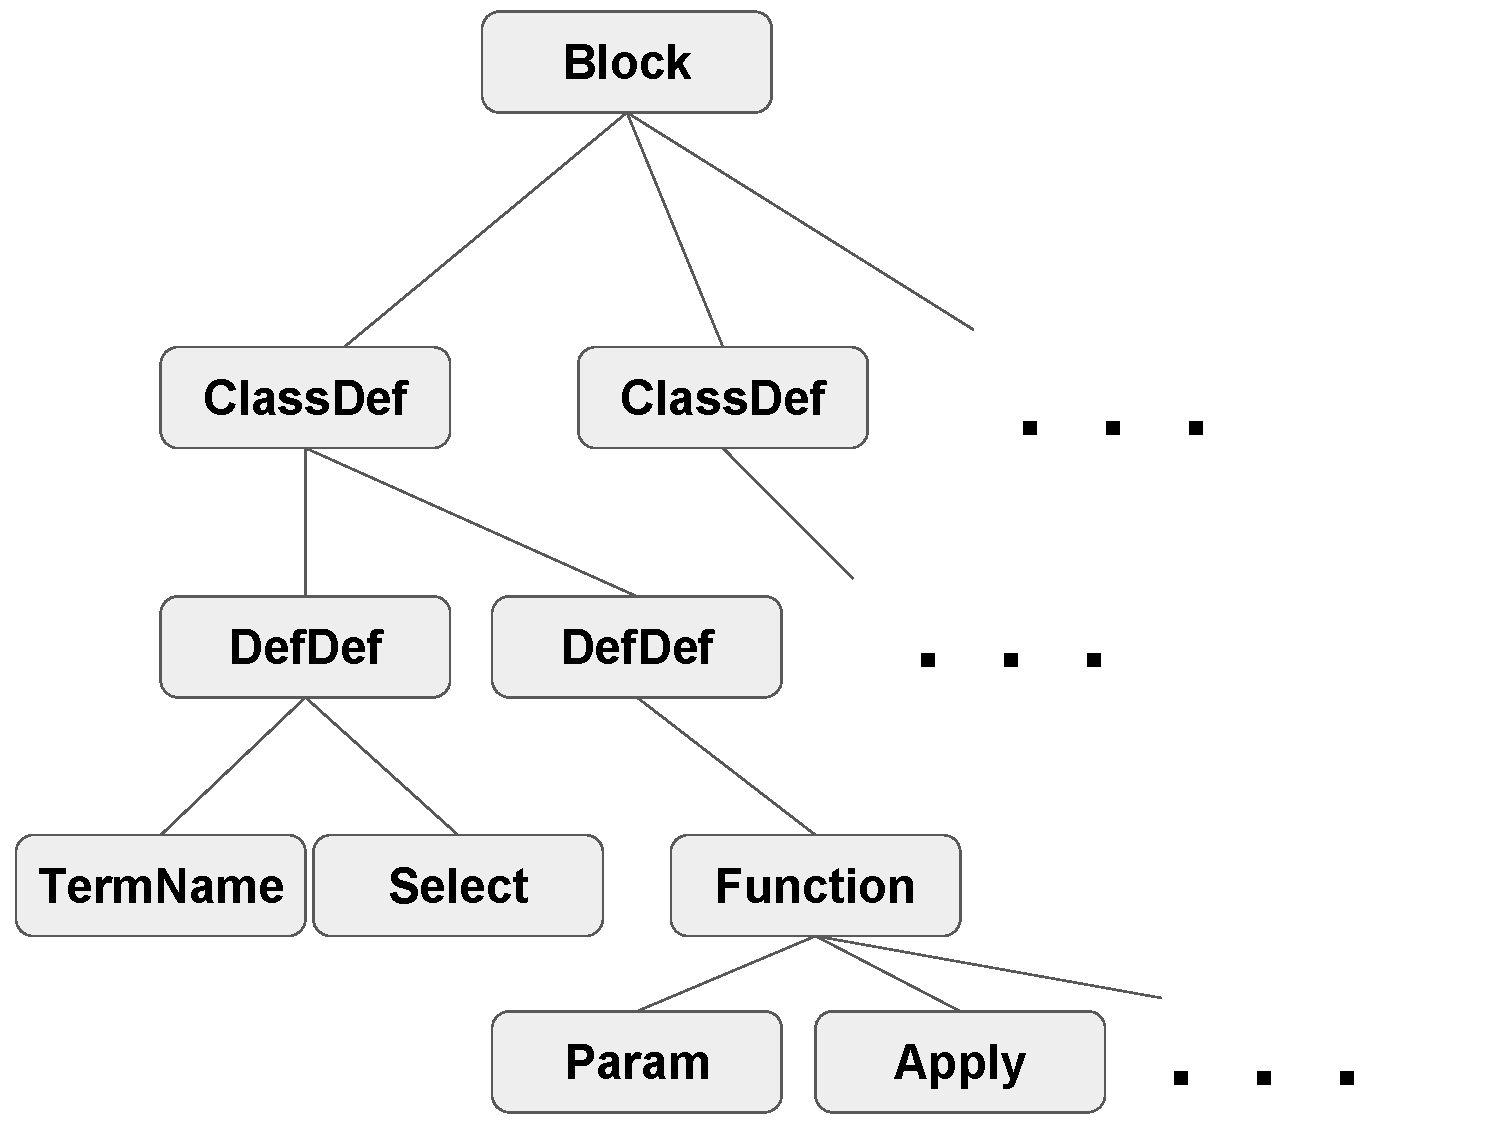
\includegraphics[width=0.4\textwidth]{image/ast}
 \caption{A sample AST with some nodes }
        \label{ast}
\end{figure}


\subsection{Tree Matching}
In this tool, we are targeting operators that are user defined and provided through the user configurations. To introduce mutations in a program, the AST of that program needs to be traversed in order to find appropriate locations (specifically nodes) where a mutation can be applied. We apply depth first search on the generated AST to find the operators and code location where the mutation should be applied. Starting with the module, this framework explores the subtree under every AST node and eventually reaches a node which is a mutation candidate. These candidates nodes are found using pattern and/or type matching of Scala. For arithmetic and boolean operators such  \texttt{+,-,>} etc, we looked for a pattern like this 
 \texttt{(SELECt(..., TERMNAME(\$plus))}  in each subtree. This search strategy works well and finds all the usage of the user defined operators that may possibly be mutated.

If a user configure the framework to work with Spark program, then we are only interested in mutating the program code that is used as closure and supplied to transformation operators. This choice of mutation location only mutates the Spark?s transformation code rather the Spark internals since the goal is to mutate that user written application. Such user written closures are detected using the pattern  \texttt{(Function(..., TERMNAME))}. This pattern cover all the UDFs in the given program and thus localize the user written code. If an AST node is found with such signature, the subtree under that node will be flagged as mutation target. By default the whole AST is flagged as non-mutation target. The implementation of this approach is flexible and can be used to localize any kind of code fragments but as of now only binary, arithmetic and UDFs based patterns are enabled. 
\subsection{Mutation Insertion}
At this point, we already have the node that is needed to be mutated. We apply the transformation as given in the user defined configuration file and replace the node with the newly generated mutated node. 
\begin{center}
\texttt{Select(b,t1,newTermName("\$minus"))-> Select(b,t1,newTermName("\$plus"))}
\end{center}
After this transformation the framework increment a newer version of the program that contains this mutant. At the end of the whole mutation process, for every mutant applied to the program, a new mutated program version would be generated. Since the mutation locations and operators are user defined, if the operator on the node is marked as the one not to be mutated then we skip the current node and move to next possible mutation location. Furthermore, in the same step we also apply the probabilistic mutation. A user defined probabilistic model is used to make a decision on whether to apply the mutation or not at the mutation candidate node. By default this model is defined in configuration as uniform distribution between 0-1.
\subsection{Refactoring and Source Code Generation}
Once we insert a mutation, the transformed AST is forwarded to refactoring and code generation module of the framework.  Since we want to keep the source code of the mutated program, we use Scala reflect library that transforms the AST into a readable source code. Keeping source code of the mutated version of the program is necessary because a user may want to compare mutation location with a fault inducing location identified from a fault localization tool. 
Converting an AST into source code is not a perfect process. The conversion from a source code into AST might lead to loss of information about the code which consequently lead to incomplete code generation when converting to source code. We rely on Scala compiler library to generate AST and to keep full information of the source code to recover it back when required. Unfortunately, the library loses information which makes is harder to generate a complete and compilable source code. In most of the cases that we observed in our subject programs, the generated source required minor cosmetic changes to make is compilable. We apply these refactoring to make the code compilable. The most frequent refactoring is the removal of  \texttt{BLOCK}  node and re-introducing package information.  \texttt{BLOCK}  node refactoring is needed because Scala compiler plugin assumes that every AST is part of a  \texttt{BLOCK}  node. The use of  \texttt{BLOCK}  node is helpful if we have multiple classes within the same file e.g  \texttt{BLOCK([class1, class2])}. The generated code  also contains the code for those  \texttt{BLOCK}  nodes. We refactor the program to remove these code fragments and transform the code into a compilable Scala code. The readable mutated code is saved into a file under the respective directory which can be built and run. 




\section{Evaluation}

\subsection{Research Questions}
We define 3 metrics for our evaluation, based on different challenges and limitations we faced with in mutation testing.
\begin{itemize} 
\item Percentage of source code files that our framework is able to mutate in each project. 
\item Percentage of created mutants which are syntactically correct
\item Percentage of tests failing on a mutant. 
\item Performance
\end{itemize}

\subsection{Subject Programs}
We are going to evaluate our framework on 5 subject programs with different code/test sizes in the later half of the project. For mid point evaluation, we only evaluated our incomplete implementation on 1 subject program. 

\subsection{Tool Applicability}

We assume that our original program is syntactically correct and compilable. Otherwise, our first and second metrics would be meaningless.  

\subsection{Tool Correctness}
We defined the first metric to measure how well our AST transformation and pattern matching process works. As for now, our algorithm is restricted to files containing one class. Second metric is measuring the effectiveness of our mutation operators and their probabilistic selection.
\subsection{Test Coverage Analysis}
Our third metric is representing quality of the test suite coverage. 
\subsection{Performance}
As for performance we are going to measure ratio of time consumed (in seconds) for mutating the program versus number of code lines. 


\section{Conclusion and Future Work}


\appendix
\section{Appendix Title}
Tool Usage 
\acks

Acknowledgments, if needed.

% We recommend abbrvnat bibliography style.

\bibliographystyle{abbrvnat}

% The bibliography should be embedded for final submission.

\begin{thebibliography}{}
\softraggedright

\bibitem[Smith et~al.(2009)Smith, Jones]{smith02}
P. Q. Smith, and X. Y. Jones. ...reference text...

\end{thebibliography}


\end{document}
